\documentclass[a4paper]{article}
%\documentclass[8pt]{report}
%%%%%%%% CREATE DOCUMENT STRUCTURE %%%%%%%%
%% Language and font encodings
\usepackage[english]{babel}
\usepackage[utf8x]{inputenc}
\usepackage[T1]{fontenc}

%\usepackage{subfig}

%% Sets page size and margins
\usepackage[a4paper,top=3cm,bottom=2cm,left=2cm,right=2cm,marginparwidth=1.75cm]{geometry}

%% Useful packages
\usepackage{amsmath}
\usepackage{graphicx}
\usepackage[colorinlistoftodos]{todonotes}
\usepackage[colorlinks=true, allcolors=blue]{hyperref}
%\usepackage{caption}
\usepackage[justification=centering]{caption}
\usepackage{subcaption}
\usepackage{sectsty}
\usepackage{float}
\usepackage{titling} 
\usepackage{blindtext}
\usepackage[square,sort,comma,numbers]{natbib}
\usepackage[colorinlistoftodos]{todonotes}
\usepackage{xcolor}
\usepackage{fancyhdr}
\usepackage{lipsum}

%% definitions 
\definecolor{darkgreen}{rgb}{0.0, 0.4, 0.0}

%% Define your personal info here %%%%%%%%%%%%%%%%%%%%%%%
\newcommand\TPid{3}
\newcommand\TPname{Simulated Annealing and Parallel Tempering for TSP}
\newcommand\Firstname{Joao Filipe}
\newcommand\Familyname{Costa da Quinta}
\newcommand\Email{Joao.Costa@etu.unige.ch}

%%%%%%%%%%%%%%%%%%%%%%%%%%%%%%%%%%%%%%%%%%%%%%%%%%%%%%%

%%%%%%% Page header %%%%%%
\pagestyle{fancy}
\fancyhf{}
\rhead{TP \TPid: \TPname}
\lhead{\Firstname \Familyname}
\rfoot{Page \thepage}


%%%%%%%% DOCUMENT %%%%%%%%
\begin{document}

%%%% Title Page
\begin{titlepage}

\newcommand{\HRule}{\rule{\linewidth}{0.5mm}} 							% horizontal line and its thickness

\center 
 
% University
\textsc{\LARGE Université de Genève}\\[1cm]

% Document info
\textsc{\Large Metaheuristics for optimization}\\[0.2cm]									% Course Code
\HRule \\[0.8cm]
{ \huge \bfseries TP \TPid : \TPname}\\[0.7cm]								% Assignment
\HRule \\[2cm]
\large
\emph{Author:} \Firstname \; \Familyname\\[0.5cm]		
\emph{E-mail:} {\color{blue}\Email}\\[7cm]		
% Author info
% Author info
{\large \today}\\[2cm]

\includegraphics[width=0.4\textwidth]{images/unige_csd.png}\\[1cm] 	% University logo
\vfill 
\end{titlepage}


% ============================================
% ----------------------------------
\newpage
\section{Introduction}
During this TP we will be working on the Travelling Salesman Problem (TSP), this is a well known problem. It consists of a Salesman that is given $n$ cities/places that he has to visit, we also assume that from any city, there is a path to visit any other city with a given distance. The goal is to find the best (shortest) path such that every city is visited exactly once, this path is also called the Hamiltonian cycle of minimal length on a fully connected graph.

\section{Simulated Annealing}
Simulated Annealing (SA) is an algorithm that is designed to copy the effect of nature itself. If a metal is heated to a certain temperature and is then cooled down progressively, the atoms reduce their movement and tend to stabilize around the minimum of energy, this method is called annealing. However, if we try to rapidly cool the same metal, the atoms won't achieve the same minimum of energy, this process is called quenching.\\\\
Intuitively, we can understand that at high temperatures the atoms aren't stable, and follow a random behaviour, therefore exploring a large number of configurations. As the temperature is reduced, the system achieves a frozen state where the atoms don't move anymore, and have achieve the, not guaranteed, global minimum.\\\\
To translate this process into an algorithm might not be obvious, but it was done. Basically what we will do, is that at the start of the exploration, we will begin with a given temperature, as high as it will ever be, which means that we allow with higher probably worst configurations than our current one to be explored. As we iterate further and further, we reduce the temperature, and will tend to accept only better configurations, until we reach a frozen state, at which point we stop.
\section{Simulated Annealing for TSP}
Let's try and apply this algorithm to TSP problem, the goal is to minimize to total length of the path while respecting the condition of visiting every city exactly once. If there are $n$ cities we want to visit, a state will be a representation of which the Travelling Salesman visits in order. $S = [1,2,3,1]$ this state means we start at city 1, go to city 2, then 3, and finally we comeback to city 1. (We want to finish were we started). In this example n = 3, but the length of our state is 4 = n + 1. The start and end are predetermined, which means the search space is $(n-1)!$, the total distance for a given path, is as follows : $\sum_{i = 1}^{n} D(s_{i}, s_{i+1})$ where $D(a,b)$ is the distance between city $a$ and $b$, the energy of a state will be represented by the total distance. A neighbour of a given state, is a simple city permutation in the path.\\\\
Let's see the flowchart/pseudocode of the algorithm:
\begin{itemize}
\item[(1)] Generate a random state S, let's call it $S\_current$
\item[(2)] Compute the initial temperature: $e^{\frac{- \langle \triangle E \rangle}{T_{0}}} = 0.5$, where $\langle \triangle E \rangle$ is the average energy change of 100 (random) neighbours of $S\_current$
\item[(3)] Set the following variables : $N\_iter = 0; N\_accept = 0$
\item[(4)] generate a new state, let this state be a random neighbour of our current state, let's call it $S\_new$, and increment $N\_iter ++$
\item[(5)] set $P = min(1, e^{\frac{- \triangle E}{T}})$, where $\triangle E = E(S\_new) - E(S\_current)$, and $T$ the current temperature, generate a random number $r$ between $0$ and $1$:
\begin{itemize} 
\item[(5.1)] if $r < P$, we set the $S\_current = S\_new$, and increment $N\_accept ++$
\item[(5.2)] if $r > P$, we keen our current state
\end{itemize}
\item[(6)] check if we are at an equilibrium state. We are at an equilibrium state if either $N\_accept = 12*n$ or $N\_iter = 100*n$
\begin{itemize} 
\item[(6.1)] if we are at an equilibrium state $\longrightarrow$ we advance to step (7)
\item[(6.2)] if we are not at an equilibrium state $\longrightarrow$ we go back to step (4)
\end{itemize}
\item[(7)] check if the system is frozen. A system is frozen if for the last three temperature changes there were no energy improvements
\begin{itemize} 
\item[(7.1)] if we are at a frozen state $\longrightarrow$ function returns $S\_current$ as the minimum
\item[(7.2)] if we are not at a frozen state $\longrightarrow$ we go back to step (3) with $T = 0.9*T$
\end{itemize}
\end{itemize}
Some notes about this algorithm, step (2) allows us to set a temperature relative to our initial random state, so for different random initial states, we will start with a different initial temperature. Step (5) makes sure we always accept a lower energy neighbour, and depending on the temperature we might accept a worst neighbour as well. The higher the temperature is, the higher probability of accepting a worse neighbour. 

\section{Results}
We will run the algorithm in a unit circle of n cities, all at the same distance from the center, so the best solution is a path in shape of a circle, and then we will run the algorithm for 2 sets of cities that are given. Finally we will generate sets of larger cities, and see what happens.\\\\
For benchmark, we will use a simple greedy algorithm, this algorithm will go from city to city, always choosing the next village as the closest one that it hasn't visited yet. This algorithm is obviously deterministic. 
\begin{figure}[H]
\center
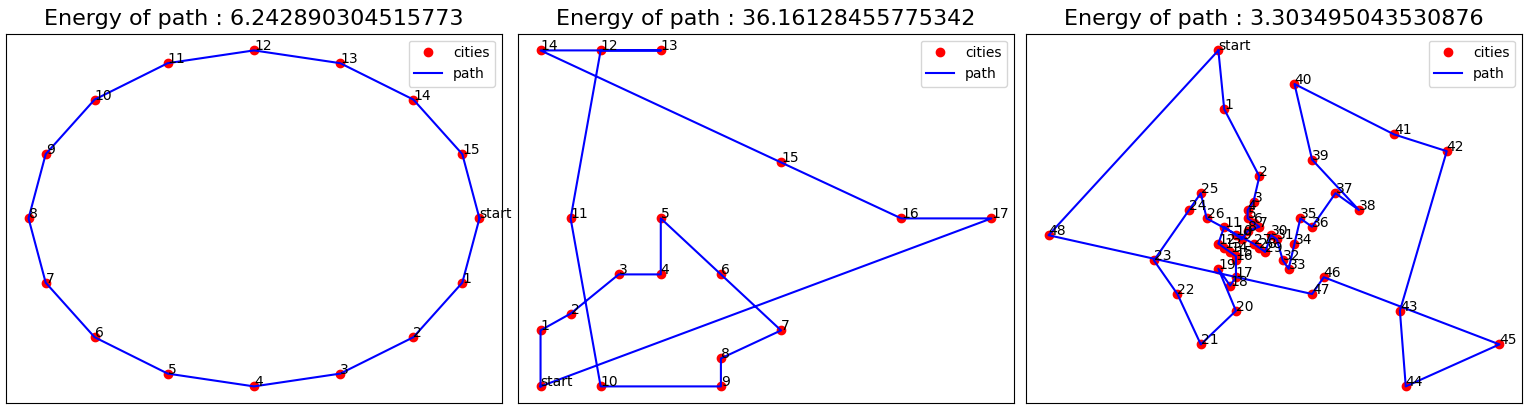
\includegraphics[width=1\textwidth]{images/algorithm_greedy.PNG}
\caption{Path found by greedy algorithm. From left to right we have : unit circle, cities.dat, cities2.dat}
\end{figure}
We can see that the algorithm only works for a perfect case scenario, and as we increase difficulty, it begins to make a mess of its path
\begin{figure}[H]
\center
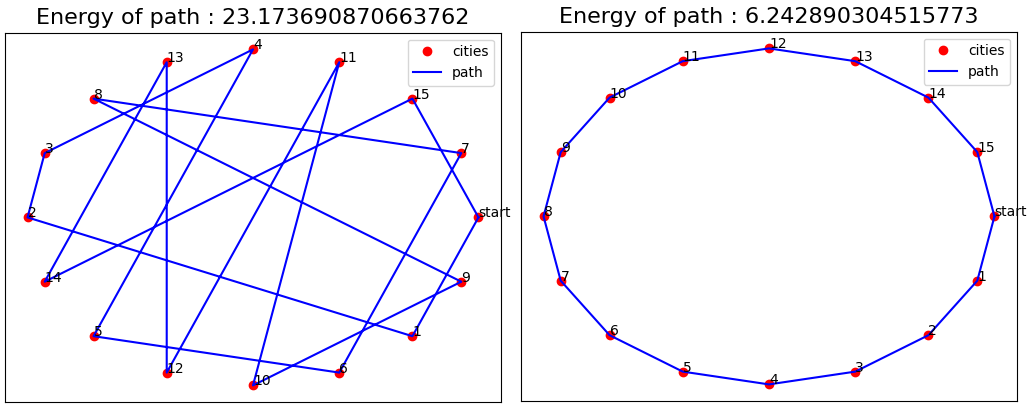
\includegraphics[width=1\textwidth]{images/algorithm_sa_circle.PNG}
\caption{Initial path and found solution found by SA algorithm for unit circle. The energy mean for 10 runs was : 6.69}
\end{figure}
\begin{figure}[H]
\center
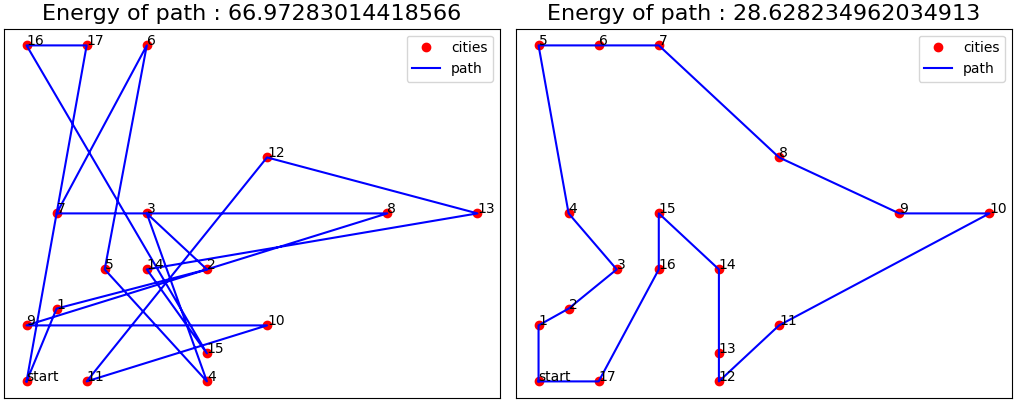
\includegraphics[width=1\textwidth]{images/algorithm_sa_cities.PNG}
\caption{Initial path and found solution found by SA algorithm for cities.dat. The energy mean for 10 runs was : 28.68}
\end{figure}
\begin{figure}[H]
\center
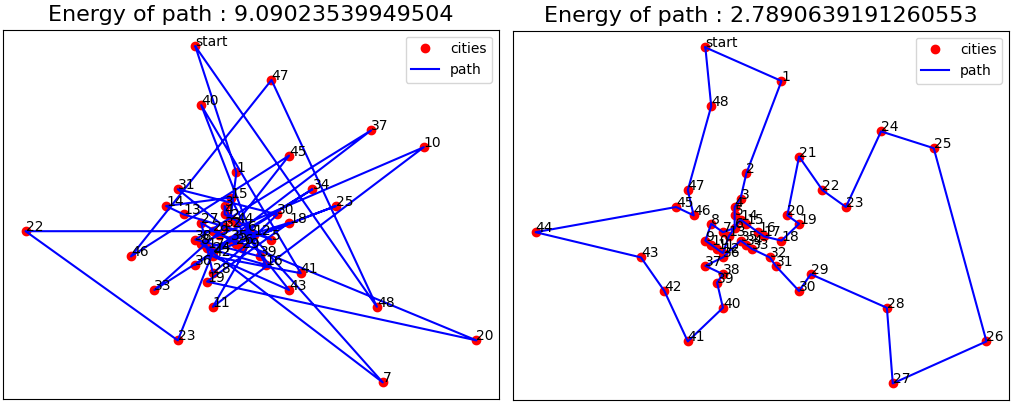
\includegraphics[width=1\textwidth]{images/algorithm_sa_cities2.PNG}
\caption{Initial path and found solution found by SA algorithm for cities2.dat. The energy mean for 10 runs was :}
\end{figure}

We see that for every case the SA algorithm performed better than the greedy. However we also notice that the mean Energy result for SA algorithm wasn't as good as the best case scenario. This is not the fault of the algorithm itself, but because of the definition of neighbourhood that we use. As we saw in class, there was another possible permutation to find neighbours, the $2-opt$, this permutation would have given better mean results for every use case.\\\\
To test our code further we had to generate a random problem of a larger size $n$.

\begin{center}
Random problem generator for $n = \{50, 100, 150\}$\\
\begin{tabular}{|c|c|c|c|}
\hline
        &  greedy algorithm &  SA best result &  SA mean result \\ \hline
 n = 50  &  136.10           &  115.85        &  123.65        \\ \hline
 n = 100 &  205.24           &  188.22    &  200.66         \\ \hline
 n = 150 &  243.78          &     240.92           &  259.68         \\ \hline
\end{tabular}
\end{center}
In every $n$ greedy algorithm was outperformed by SA, it must be noted that SA had difficulties with $n = 150$, and it's mean result is actually worse than greedy algorithm, out of 10 executions, only one was better than greedy algorithm. We have to take into account that the 150 cities were all in a plane of 20 by 20, which means there wasn't actually many possibilities for the greedy algorithm to go wrong, my assumption is that in a larger plane greedy algorithm wouldn't be as accurate. This being said, I didn't rerun the simulation in a larger plane as it took way too long.\\\\
We do have to take into account the complexity of both algorithms, greedy has a time complexity of $O(2n)$, however SA algorithm has a much higher time complexity. If we look back at the flowchart of the algorithm, step (4) was iterated at least $n^{2}$ times, which means the complexity is at least $O(n^{2})$.\\\\
With all the results having been discussed, I must admit I was very impressed at how well the algorithm performed, and how it was capable to optimize the path while trying to emulate a real physical process found in nature.
\end{document}
